\documentclass[11pt,openany]{templcl}
% \documentclass[en,11pt]{aghdpl}  % praca w języku angielskim
\usepackage[polish]{babel}
%\usepackage[english]{babel}
\usepackage[utf8]{inputenc}

% dodatkowe pakiety
\usepackage{enumerate}
\usepackage{listings}
\lstloadlanguages{TeX}

\lstset{
  literate={ą}{{\k{a}}}1
           {ć}{{\'c}}1
           {ę}{{\k{e}}}1
           {ó}{{\'o}}1
           {ń}{{\'n}}1
           {ł}{{\l{}}}1
           {ś}{{\'s}}1
           {ź}{{\'z}}1
           {ż}{{\.z}}1
           {Ą}{{\k{A}}}1
           {Ć}{{\'C}}1
           {Ę}{{\k{E}}}1
           {Ó}{{\'O}}1
           {Ń}{{\'N}}1
           {Ł}{{\L{}}}1
           {Ś}{{\'S}}1
           {Ź}{{\'Z}}1
           {Ż}{{\.Z}}1
}

%---------------------------------------------------------------------------

\author{Grzegorz Bylina, Agata Paciorek}
\shortauthor{G. Bylina, A. Paciorek}

\titlePL{\textbf{mHealth}}
\titleEN{Thesis in \LaTeX}

\shorttitlePL{mHealth} % skrócona wersja tytułu jeśli jest bardzo długi
\shorttitleEN{Thesis in \LaTeX}

\thesistype{Systemy informatyczne w medycynie - raport}
%\thesistype{Master of Science Thesis}

%\supervisor{dr hab. Marcin Szpyrka, prof. n.}
%\supervisor{Marcin Szpyrka PhD, DSc}

\degreeprogramme{Informatyka}
%\degreeprogramme{Computer Science}

\date{2014}

\department{Katedra Informatyki Stosowanej}
%\department{Department of Applied Computer Science}

\faculty{Wydział Elektrotechniki, Automatyki,\protect\\[-1mm] Informatyki i Inżynierii Biomedycznej}
%\faculty{Faculty of Electrical Engineering, Automatics, Computer Science and Biomedical Engineering}



\setlength{\cftsecnumwidth}{10mm}

%---------------------------------------------------------------------------

\begin{document}

\titlepages

\tableofcontents

\chapter{Wstęp teoretyczny}
Koncepcja \textbf{M-Health} (\emph{Mobile Health}) jest integracją mobilnej telekomunikacji i technologii multimedialnej, której celem jest dostarczanie opieki zdrowotnej.\\
Zadania M-Health \cite{5969916} :
\begin{itemize}
\item zbieranie danych klinicznych
\item dostarczanie informacji do personelu medycznego, badaczy, pacjentów
\item monitorowanie pacjenta real-time
\item dostarczanie opieki medycznej
\end{itemize}
Mobile Health zajmuje się dostarczaniem opieki wszędzie i o każdej porze, surpassing geographical, temporal, even organizational barier \cite{6655256}. Nie kończy się (m-health) na udostępnianiu aplikacji opieki zdrowotnej na urządzeniach mobilnych as m-health can involve czujniki i sieci bezprzewodowe, urządzenia mobilne do dostępu do variety of usług medycznych, profesjoalistów w celu podjęcia decyzji i dostarczaniu opieki zdrowotnej i zarządzaniu aktywności dla osób starszych \cite{Varshney2014}.Weź to popraw człowieku zeby nie bylo żywcem z artykulu.

\chapter{Przykłady rozwiązań}
\section{Monitorowanie pacjenta}
\paragraph{Monitorowanie postury \cite{Lee:2012:MPM:2370216.2370320}\\}
Zaproponowany mechanizm szacuje różne wartości reprezentujące posturę użytkownika takie jak: kąt nachylenia szyi , odległość oglądania, stan wzroku użytkownika poprzez analizę danych z przedniej kamery , akcelerometru, czujnika orientacji lub dowolną ich kombinację. Powiadamia użytkownika jeśli oszacowane
wartości są utrzymywane w nieprawidłowym zakresie ponad dozwolony czas.
\paragraph{Ocena zdrowia i zdolności kierowcy \cite{6583819}\\}
Aplikacja sprzężona z Data Loggerem zainstalowanym w pojeździe, który gromadzi dane z czujników znajdujących się w pojeździe i na ciele kierowcy. Aplikacja jest przeznaczona do monitorowania jakości sygnałów real-time i znacznego skrócenia czasu oszacowania stanu zdrowia kierowcy łącznie z jego zdolnościami do prowadzenia pojazdów. System składa się z dwóch modułów:
\begin{itemize}
\item smartbio 1 - system badania\\
Służy do ułatwienia gromadzenia informacji na temat rożnych badań fizjologicznych/psychologicznych i wykorzystanie ich do obliczenia współczynnika, określającego zdolność kierowcy do jazdy

\item smartbio 2 - system monitorowania\\
Dzieli się na dwie warstwy hardware i monitoring. Warstwa hardware gromadzi i wstępnie przetwarza dane (z sensorów). Warstwa monitoring ma postać aplikacji na smartfona, jej głównym zadaniem jest komunikacja między użytkownikiem, a warstwą hardware
\end{itemize}
\paragraph{Diagnozowanie depresji\\}
 Ta praca prponuje techniki poprawiające komunikacje w BSN (Body Sensor Network), które gromadzą dane o stanach emocjonalnych pacjenta. 
 Te BSN  mogą stale monitorować , dyskretnie szacować i klasyfikować każdy stan depresyjny. Dodatkowo dane na temat życia pacjenta mogą zostać skorelowane z 
 uwarunkowaniami fizjologiczymi aby zidentyfikować jak poszczególne bodźce wywołują objawy. Taki ciągły strumień danych jest poprawą w stosunku do 
 migawki objawów , które zaobserwuje lekarz w ciągu badania. 
 
 
\section{Zarządzanie informacją}
\paragraph{Zarządzanie chorobami przewlekłymi\\}
Jest to pewna znaleziona koncepcja aplikacji mobilnej. Celem pracy było zidentyfikowanie funkcji i wymagań funkcyjnych , które pomogły by użytkownikowi w zarządzaniu opieką nad swoją chorobą przewlekłą
 Projekt przewiduje kompleksowe działania takie jak wyświetlanie i zarządzanie lekami, harmonogram badań/wizyt, notatki, plany diet, ważne informacje o planie leczenia

\paragraph{Zarządzanie lekami\\}
 Aplikacja do zarządzania podawaniem leków. To pamiętnik śledzący i zarządzający lekami w celu zapobiegania błędom medycznym. 
 Poprzez wizje,dźwięk,wibracje  SapoMed przypomina użytkowników o ich harmonogramie leków
 Aplikacja umożliwia rejestrowanie leków poprzez kamerę za pomocą barcode na opakowaniu. 
 Korzysta z usług internetowych (web services) aby uzyskać informacje o lekach a nawet o ich dawkowaniu
 Wykorzystuje te web services również do zapamiętywania spożywanych wczesniej leków 
\section{Problem bezpieczeństwa}
\chapter{Zastosowania}
\chapter{Podsumowanie}
\chapter{Przykłady rozwiązań}
\label{cha:przyklady_rozw}

\section{Monitorowanie pacjenta}
\label{sec:monitorowanie_pacj}
\subsection{Monitorowanie postury \cite{Lee:2012:MPM:2370216.2370320}}
Zaproponowany mechanizm szacuje różne wartości reprezentujące posturę użytkownika takie jak: kąt nachylenia szyi , odległość oglądania, stan wzroku użytkownika poprzez analizę danych z przedniej kamery , akcelerometru, czujnika orientacji lub dowolną ich kombinację. Powiadamia użytkownika jeśli oszacowane
wartości są utrzymywane w nieprawidłowym zakresie ponad dozwolony czas.

\subsection{Ocena zdrowia i zdolności kierowcy \cite{6583819}}
Aplikacja sprzężona z Data Loggerem zainstalowanym w pojeździe, który gromadzi dane z czujników znajdujących się w pojeździe i na ciele kierowcy. Aplikacja jest przeznaczona do monitorowania jakości sygnałów real-time i znacznego skrócenia czasu oszacowania stanu zdrowia kierowcy łącznie z jego zdolnościami do prowadzenia pojazdów. System składa się z dwóch modułów:
\begin{itemize}
\item smartbio 1 - system badania\\
Służy do ułatwienia gromadzenia informacji na temat rożnych badań fizjologicznych/psychologicznych i wykorzystanie ich do obliczenia współczynnika, określającego zdolność kierowcy do jazdy

\item smartbio 2 - system monitorowania\\
Dzieli się na dwie warstwy hardware i monitoring. Warstwa hardware gromadzi i wstępnie przetwarza dane (z sensorów). Warstwa monitoring ma postać aplikacji na smartfona, jej głównym zadaniem jest komunikacja między użytkownikiem, a warstwą hardware
\end{itemize}

\subsection{Diagnozowanie depresji \cite{5291726}}
 
Ta praca proponuje techniki poprawiające komunikacje w BSN (Body Sensor Network), które gromadzą dane o stanach emocjonalnych pacjenta. BSN  mogą stale monitorować, dyskretnie szacować i klasyfikować stany depresyjne. Dodatkowo dane na temat życia pacjenta mogą zostać skorelowane z uwarunkowaniami fizjologicznymi, aby zidentyfikować w jaki sposób poszczególne bodźce wywołują objawy. Taki ciągły strumień danych jest poprawą w stosunku do migawki objawów, które zaobserwuje lekarz w ciągu badania. 
 

%---------------------------------------------------------------------------

\section{Zarządzanie informacją}
\label{sec:zarzadz_inf}

\subsection{Zarządzanie chorobami przewlekłymi}
Jest to pewna znaleziona koncepcja aplikacji mobilnej. Celem pracy było zidentyfikowanie funkcji i wymagań funkcyjnych , które pomogły by użytkownikowi w zarządzaniu opieką nad swoją chorobą przewlekłą
 Projekt przewiduje kompleksowe działania takie jak wyświetlanie i zarządzanie lekami, harmonogram badań/wizyt, notatki, plany diet, ważne informacje o planie leczenia

\subsection{Zarządzanie lekami}
 Aplikacja do zarządzania podawaniem leków. To pamiętnik śledzący i zarządzający lekami w celu zapobiegania błędom medycznym. 
 Poprzez wizje,dźwięk,wibracje  SapoMed przypomina użytkownikom o ich harmonogramie leków.
 Aplikacja umożliwia rejestrowanie leków poprzez kamerę za pomocą barcode na opakowaniu. 
 Korzysta z usług internetowych (web services) aby uzyskać informacje o lekach, a nawet o ich dawkowaniu
 Wykorzystuje też web services do zapamiętywania spożywanych wcześniej leków.

\section{Problem bezpieczeństwa}
\label{sec:problem_bezp}
Zgodnie z pracą \cite{Ammar2014}, aplikacje mobilne zbierają dane z wszechobecnych urządzeń i łączą je z innymi danymi o użytkownikach w różnych celach. Atomicznie, te źródła danych nie muszą ujawniać danych osobowych dla osób fizycznych, lecz połączenie wielu rozproszonych źródeł może doprowadzić do niezamierzonych konsekwencji i naruszyć prywatność. Według raportów rządowych około osiem milionów rekordów danych zdrowotnych pacjentów wyciekły w ciągu ostatnich kilku lat. Zachodzi więc potrzeba dostarczenia odpowiednich infrastruktur, aby przekonać użytkowników do dzielenia się danymi. 

\subsection{Privacy management framework \cite{Ammar2014}}
W pracy zostaje zaproponowany framework zarządzania prywatnością dla mobilnych aplikacji opieki zdrowotnej z wsparciem dla dynamicznego zarządzania prywatnością dzielenia danych. Rozwiązanie to rozszerza XACML poprzez wprowadzenie kontekstu dostępu użytkownika do egzekwowania zasad prywatnej polityki. Dostarczona zostaje implementacja, budująca na platformie Google App Engine.


\chapter{Zastosowania}
\label{cha:zastosowania}

\section{Choroby serca i pierwsza pomoc przy zawale}

Obecne społeczeństwo najwięcej kłopotów zdrowotnych ma z układem krążenia. Choroby serca są najbardziej rozpowszechnione na świecie, zwłaszcza w krajach wysoko rozwiniętych. Dlatego niezmiernie ważne jest nie tylko leczenie, ale także i zapobieganie chorobom i rehabilitacja po zawale.
\subsection{Telefony komórkowe a pierwsza pomoc}

W przypadku zawału serca niezbędna jest szybka reakcja. Często jednak stres uniemożliwia poprawne udzielenie pierwszej pomocy. Z pomocą przychodzą nam coraz szerzej dostępne inteligentne telefony komórkowe - smartphone'y. W czasopiśmie "Interventional Cardiology" (\cite{ICHoneyman2014Mobilehealthapplicationsincardiaccare}) opisane jest, w jaki sposób aplikacja mobilna może pomóc w przeprowadzeniu akcji rehabilitacyjnej:
\begin{figure}[ht!]
  \centering
    \reflectbox{%
      \includegraphics[width=0.5\textwidth]{images/cpr}}
  \caption{Schemat akcji resuscytacyjnej przy pomocy smartphone'a}
\end{figure}

\subsection{Pomoc po zawale}

Po zawale serca bardzo ważna jest praca nad stanem układu krążenia. Często jednak odległość do najbliższego szpitala jest czynnikiem zaporowym, uniemożliwiającym poprawne zadbanie o zdrowie. Ostatnie badania pokazują jednak \cite{FMottl2014Smartphoneappprovesvaluableforcardiacpatients}, iż telefon komórkowy może znacznie poprawić sytuację pacjentów pozawałowych. Aplikacja przypomina o regularnych ćwiczeniach i pozwala monitorować aktualny stan zdrowia.
\section{Monitorowanie pacjenta chorego na cukrzycę}
\label{sec:cukrzyca}

Problem cukrzycy jest również jednym z najpoważniejszych zadań, z jakimi spotyka się dzisiejsza medycyna. Dotyczy on bowiem znacznej części społeczeństwa. W artykule \cite{CDTran2012Smartphone-BasedGlucoseMonitorsandApplicationsintheManagementofDiabetes:AnOverviewof10SalientAppsandaNovelSmartphone-ConnectedBloodGlucoseMonitorUnitedStates--USGlucoseSmartphonesCellulartelephonesDiabetes} możemy znaleźć informacje na temat dostępnych na rynku aplikacji do monitorowania poziomu cukru we krwi.
\subsection{Przegląd aplikacji}
Na rynku dostępnych jest wiele aplikacji na wszystkie popularne obecnie platformy, takie jak Android, iOS czy BlackBerry OS.
\paragraph{Glucose Buddy}\mbox{}\\
Aplikacja firmy SkyHealth integruje funkcjonalność smartphone'a z danymi dostępnymi w internecie. Użytkownik może śledzić nie tylko swój poziom cukru we krwi, ale także na przykład ilość przyjmowanych składników spożywczych. Aplikacja jest darmowa.
\paragraph{Diabetes Buddy}\mbox{}\\
Płatną, ale bardziej rozwiniętą aplikacją, jest Diabetes Buddy. Umożliwia ona także monitorowanie poziomu ciśnienia krwi.
\paragraph{Log Frog}\mbox{}\\
Jedną z ciekawszych propozycji na rynku jest aplikacja Log Frog. Oferuje ona opisane wcześniej funkcjonalności, różni się jednak bardzo przyjaznym i prostym interfejsem, odpowiednim dla dzieci bądź osób starszych.

\section{Aplikacja mobilna a choroby psychiczne}
Okazuje się, iż telefony komórkowe obecnie mogą pomóc nie tylko osobom chorym z powodu dysfunkcji narządów. Także pacjenci mentalnie chorzy mogą liczyć na pomoc dzisiejszej technologii. Za pomocą odpowiednich systemów monitorowane są ich zachowania w konkretnych sytuacjach, przez co osobom opiekującym się nimi łatwiej jest dostrzec nieprawidłowości.\\
Do tej pory prowadzone badania obejmowały m. in. schizofrenię i psychozę oraz chorobę dwubiegunową \cite{IJOMHSPawelProciow2012Mobilepsychiatry:towardsimprovingthecareforbipolardisorderScience&TechnologyLifeSciences&BiomedicinePsychiatryPSYCHIATRYSSCIAMBULATORYASSESSMENTCIRCADIAN-RHYTHMSMENTAL-DISORDERSDAILY-LIFEPSYCHOLOGYCREATIVITYMOVEMENTBURDENSLEEP}. W artykule \cite{JoPNHSElias2014MobileAppsforPsychiatricNursesPsychiatric-mentalhealthnursingSmartphonesHandheldcomputersSoftware} omówione zostały aplikacje przydatne specjalistom w dziedzinie psychologii. \\ \\ \\
\begin{figure}[ht!]
  \centering
    \reflectbox{%
      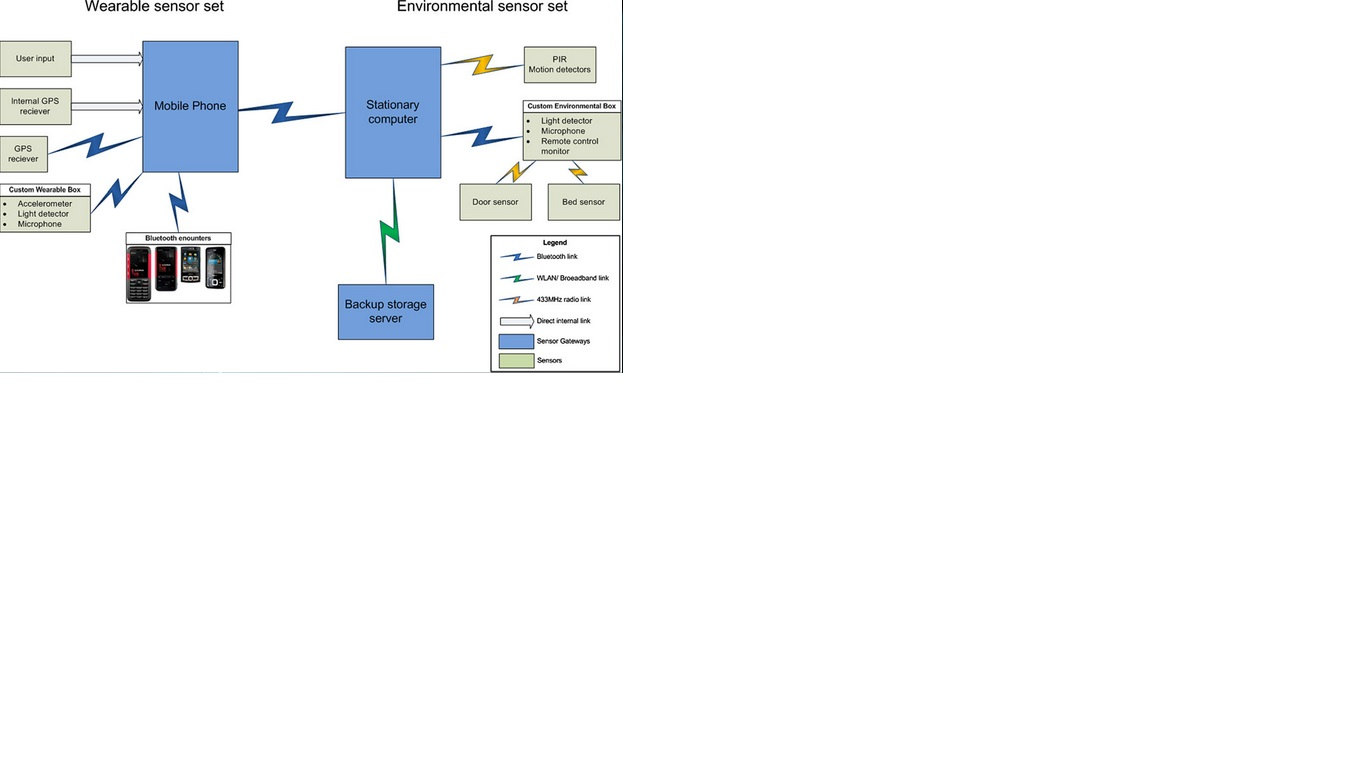
\includegraphics[width=0.5\textwidth]{images/psychic}}
  \caption{Schemat aplikacji badającej zachowania pacjenta chorego psychicznie}
\end{figure}
\section{Akcelerometr  w leczeniu choroby parkinsona}
Również choroby neurodegeneracyjne mają swoją szufladę w dziedzinie rozwoju technologii mHealth. Badania pokazują (\cite{AICPSSanders2013RemotesmartphonemonitoringformanagementofParkinsonsDiseaseEEGaccelerationactivitymonitoringelectroencephalogrammobilecomputingsensorsmart-phonewatchwrist}), iż regularne monitorowanie stanu zdrowia pacjenta może znacznie opóźnić rozwój choroby. Niestety częste wizyty w szpitalu dla wielu pacjentów są nieomal nieosiągalne. Dlatego też podręczne urządzenia, takie jak smartphone'y, okazują się tu nieocenione. Jeden z największych koncernów - Intel \cite{BMacKellar2014AussiemhealthfirmtorollouttoolforParkinsons} - pracuje nad technologią przenośnych "gadżetów", które chory mógłby nosić w celu monitorowania stanu zdrowia.
\section{Leczenie i kontrolowanie uzależnień}
Kolejnym z problemów, z jakim spotyka się obecna medycyna, jest uzależnienie od leków. Nadużywanie przepisanych medykamentów, co dotyczy zwłaszcza opioidów, nie tylko podwyższa koszty leczenia, ale także może prowadzić do poważnych zaburzeń zdrowotnych. W rezultacie pacjent zamiast się leczyć, pogarsza tylko swoją sytuację. Aby temu zapobiec, można skorzystać z pomocy urządzeń mobilnych. Monitorowanie przyjmowania odpowiednich dawek leków, czy to poprzez wprowadzanie danych przez pacjenta, czy nawet dzięki urządzeniom pomiarowym, noszonym przy ciele, może pomóc wykryć pewne wzorce, wskazujące na wysokie ryzyko, iż terapia może zakończyć się uzależnieniem \cite{ISoMAHN&CVarshney2014Mobilehealth:medicationabuseandaddictionaddictionmobilehealthmonitoringprescriptionabuse}.\\
Na rysunku \ref{fig:drugs} ukazany jest przykładowy schemat takiej aplikacji.
\\ \\ \\ \\
\begin{figure}[ht!]
  \centering
    \reflectbox{%
      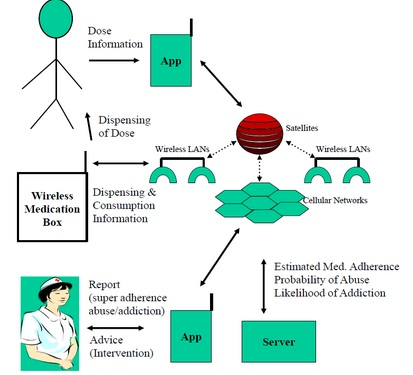
\includegraphics[width=0.5\textwidth]{images/drugs}}
  \caption{Schemat aplikacji do detekcji uzależnienia od leków}
  \label{fig:drugs}
\end{figure}

\section{Mobilna opieka nad ciążą}
W miejscach, gdzie opieka medyczna nie jest ogólnodostępna, ciąża wiąże się z ogromnym ryzykiem powikłań, które, nieleczone, często prowadzą do zgonu zarówno matki, jak i dziecka. Ponieważ technologia komórkowa w obecnych czasach jest już nieomal w stu procentach powszechna, postanowiono wykorzystać ją do pomocy przyszłym matkom, nie mogącym sobie pozwolić na częste wizyty w szpitalu. Dzięki telefonii komórkowej kobiety mogą otrzymywać nie tylko informacje o prawidłowym rozwoju ciąży i instrukcje, jak samodzielnie badać, czy dziecko rozwija się poprawnie, ale także i szybszą pomoc - istnieje specjalny system \cite{Ismaeel2013EffectiveSystemforPregnantWomenusingMobileGIS} oferujący szybką pomoc kobietom, którym grozi ryzyko poronienia, a nawet śmierci. Dzięki usługom lokalizacyjnym nawet w przypadku utraty przytomności matka ma szansę otrzymać pomoc na czas.
\begin{figure}[ht!]
  \centering
    \reflectbox{%
      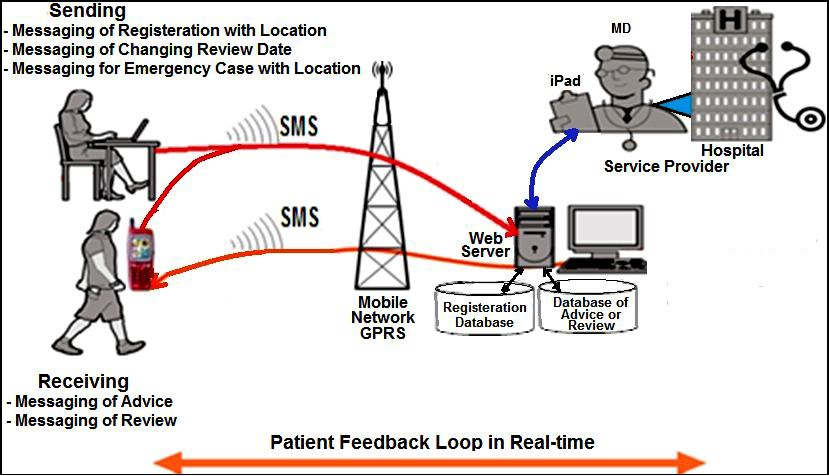
\includegraphics[width=0.5\textwidth]{images/pregnancy}}
  \caption{Budowa systemu powiadamiania i konsultacji medycznych dla kobiet w ciąży}
\end{figure}
\chapter{Podsumowanie}
\label{cha:podsumowanie}
\chapter{Ściąga z artykułami}
\label{cha:sciaga}

\cite{JoMIRPalmert2012DesignofanmHealthAppfortheSelf-managementofAdolescentType1Diabetes:APilotStudy} Artykuł traktuje o zastosowaniu aplikacji m-health przy schorzeniach cukrzycy typu 1 (nieinsulinozależnej). Ponieważ dla cukrzyków typu 2 aplikacje te wykazały bardzo dużą poprawę stanu zdrowia i świadomości użytkowników, postanowiono zbadać, jak sytuacja przedstawia się dla osób chorujących na cukrzycę typu 2.
\cite{IENEleanorS.Freshwater2014Technologyfortrauma:testingthevalidityofasmartphoneappforpre-hospitalclinicians} W tym artykule omówiona jest skuteczność aplikacji na smartphone'a w kwestii przydzielania pacjentów po urazie do odpowiednich placówek hospitalizacyjnych. Porównana jest ona z tradycyjną metodą, wymyśloną na potrzeby „sieci urazowej”, stworzonej w Anglii.
\cite{AjopDavidKimhy2014Useofmobileassessmenttechnologiesininpatientpsychiatricsettings} Przeprowadzono test użyteczności aplikacji m-health dla pacjentów cierpiących na poważne zaburzenia psychiczne – w tym wypadku schizofrenii. Badano wartość informacji uzyskanych dzięki takiej aplikacji w kontekście wartości medycznej.
\cite{JomIrBierbrier2014EvaluationoftheAccuracyofSmartphoneMedicalCalculationApps} Ponieważ dokładność aplikacji pracujących na danych medycznych nie była nigdy obliczana, postanowiono ją zbadać. Przetestowano ogólnodostępne aplikacje z takich serwisów jak Google Play, BlackBerry World i iTunes App Store.
\cite{MPiEKer-Cheng2014ASmartphoneAPPforHealthandTourismPromotionSmartphones;Tourism;Colleges&universities;Marketing;Historicbuildings&sites;Festivals;Parks&recreationareas;Onlineinstruction;Folklore;Scienceeducation;Ruralareas;Mountainclimbing} Tematem pracy jest aplikacja, której celami są edukacja , promocja turystyki oraz promocja zdrowia poprzez monitorowanie zużycia energii użytkownika.
\cite{AICPSSanders2013RemotesmartphonemonitoringformanagementofParkinsonsDiseaseEEGaccelerationactivitymonitoringelectroencephalogrammobilecomputingsensorsmart-phonewatchwrist} Monitorowanie choroby Parkinsona na podstawie badań prowadzonych w domu przy pomocy telefonu komórkowego typu smartphone oraz wykorzystywanie zebranych danych do efektywniejszej terapii.
\cite{POChaiyachati2013APilotStudyofanmHealthApplicationforHealthcareWorkers:PoorUptakeDespiteHighReportedAcceptabilityataRuralSouthAfricanCommunity-BasedMDR-TBTreatmentProgramHospitals;Tuberculosis;Studies;Intervention;Workers;Patients} Praca mówi o aplikacji do monitorowania pacjentów z gruźlicą oporną na wiele leków. Jej celem jest ocena działania aplikacji
\cite{BCDPfaeffli2012AmHealthcardiacrehabilitationexerciseintervention:findingsfromcontentdevelopmentstudiesCardiacrehabilitation;Exercise;Telemedicine;Internet}Stworzenie aplikacji mobilnej wspomagającej program „rehabilitacji serca” (cardiac rehabilitation) i badanie jej efektywności wśród pacjentów objętych tym programem.
\cite{BIRajan2012ThePromiseofWireless:AnOverviewofaDevice-To-CloudmHealthSolutionControlInstrumentationSurgicalimplantsMonitoringBusinessJourneysHealthcareSubsidiaries} Artykuł traktujący o tworzeniu i użytkowaniu aplikacji m-health, a także problemach i korzyściach wynikających z zastosowania technologii chmury.
\cite{ICHoneyman2014Mobilehealthapplicationsincardiaccare} Przegląd zastosowań aplikacji m-health dla osób cierpiących na przewlekłe choroby serca, takie jak np. arytmia. Zwrócenie uwagi na pomoc aplikacji w zwiększeniu świadomości w dziedzinie pierwszej pomocy przy atakach serca.
\cite{BISikka2012TheFutureofMedicine:TheEmergencyRoomAndMobileHealthInstrumentationTrackingMonitoringEmergenciesHealthcareHealthEmergencymedicalservicesHospitals} Wywiad ze specjalistami w dziedzinie m-health, wskazującymi na korzyści wynikające z globalnego zastosowania medycznych aplikacji mobilnych, takich jak np. wcześniejsza diagnoza w przypadku ataku osoby chorej na serce czy lepszy styl życia u osób chorych na cukrzycę, pozwalający zdecydowanie zmniejszyć terapię farmakologiczną.
\cite{MEPeck2012LivelifeuntetheredwithmobilehealthappsUnitedStates--USPhysiciansSmartphonesCellularPhonePhysiciansPrimaryCareSoftwareutilitiesHumansUnitedStatesElectronichealthrecordsPracticeManagementMedicalPortablecomputersMedicalInformaticsSoftware} Przedstawiony jest tu punkt widzenia lekarza korzystającego z aplikacji. Omówione są wszystkie udogodnienia, jakie oferuje korzystanie z telefonu w codziennej pracy.
\cite{PPRModi2013MobileHealthTechnologyinDevelopingCountries:TheCaseofTanzaniaWorldHealthOrganizationTanzaniaPublichealthHumanimmunodeficiencyvirus--HIVAcquiredimmunedeficiencysyndrome--AIDSCellulartelephonesDevelopingcountries--LDCs} Badanie wpływu użytkowania aplikacji m-health we wschodnioafrykańskiej Tazanii, gdzie istnieje duże ryzyko zarażenia rozmaitymi chorobami, także przewlekłymi. Teza, iż poprawa stanu zdrowia w kraju pozwoli na prężniejszy rozwój ekonomiczny.
\cite{PMFree2012TheEffectivenessofMobile-HealthTechnology-BasedHealthBehaviourChangeorDiseaseManagementInterventionsforHealthCareConsumers} Analiza korzyści wynikających z użytkowania medycznych aplikacji mobilnych w codziennym życiu – dane statystyczne, zgromadzone z wielu źródeł
\cite{PDaTMurad2014TheimpactofmobilehealthapplicationsonemergencymedicalservicesandpatientinformationprivacyHealthcaremanagementGeographicinformationscienceComputerscienceInformationTechnology} Autor zwraca uwagę na fakt, iż w większości aplikacji zdrowotnych sprawa prywatności i bezpieczeństwa danych użytkowników traktowana jest drugorzędnie, jako dodatek do aplikacji. Badana jest tu także metoda jak najefektywniejszej wymiany danych.
\cite{Bi&t/AftAoMILogan2012ARoundtableDiscussion:EmbracingtheMobileRevolutionIndexMedicus} Rozmowa z ekspertami w dziedzinie zdrowia i technologii bezprzewodowych. Poruszono takie kwestie jak odpowiednie urządzenia, połączenie aplikacji bezpośrednio ze szpitalem oraz przyczynę popularyzowania się technologii mHealth
\cite{NEPSkiba2014TheConnectedAge:MobileAppsandConsumerEngagementSmartphonesInternetaccessFDAapprovalDiseasecontrolElectronichealthrecordsHumansInformationmanagementStudentsNursingConsumerParticipationPatientsTextmessagingSocialnetworksWomenshealthHospitalsPersonalhealthGlobalpositioningsystems--GPS} Próba skierowania zainteresowania użytkowaniem smartphone'ów studentów (i nie tylko) w kierunku technologii wspomagających zachowania sprzyjające utrzymaniu dobrego stanu zdrowia.
\cite{PDaTWerkmeister2013TheUseofApplicationsonMobileDevicesinaMidwesternPopulationClinicalpsychologyPsychology} Analiza popularności użytkowania aplikacji mobilnych wśród osób cierpiących na różne problemy zdrowotne – jak choćby depresja czy dysfunkcje wynikające z nadużywania alkoholu
\cite{BIFacchinetti2012ThisProcessIsJustBeginning:ConnectingMobileMedicalDevicesTelemedicineWirelessTechnologyTechnologicalchangeDeliveryofHealthCareComputerCommunicationNetworksSystemsIntegrationMedicalequipmentInformationtechnologySoftware} Nieustannie postępujący rozwój technologii zmusza autorów artykułu do przeanalizowania przyszłości urządzeń medycznych pod kątem ich całkowitego połączenia, także w dziedzinie wymiany informacji, w przeciwieństwie do obecnej architektury bazującej na indywidualnych topologiach maszyn.
\cite{Ismaeel2013EffectiveSystemforPregnantWomenusingMobileGIS} Ze względu na dużą śmiertelność wśród ciężarnych kobiet w krajach, gdzie opieka medyczna nie jest ogólnodostępna, takich jak Afryka czy Azja, postanowiono zaproponować rozwiązanie problemu bazujące na aplikacji mHealth.
\cite{CDRJ.GrahamThomas2014ReviewofInnovationsinDigitalHealthTechnologytoPromoteWeightControlScience&TechnologyLifeSciences&BiomedicineEndocrinology&MetabolismENDOCRINOLOGY&METABOLISMRANDOMIZED-CONTROLLED-TRIALPHYSICAL-ACTIVITYLOSSPROGRAMLOSSMAINTENANCEMOBILE-TECHNOLOGYOBESITYEPIDEMICECONOMICBURDENUNITED-STATESPRIMARY-CAREUSADULTS} Postęp technologiczny w ostatnich latach spowodował drastyczny wzrost problemów zdrowotnych społeczeństwa wynikających z otyłości. Postanowiono wykorzystać ten rozwój na korzyść większej kontroli wagi wśród osób używających smartphone'ów na co dzień.
\cite{FMottl2014mHealthappoffersround-the-clockmedicalconciergesubscriptionservice} Opis nowo udostępnionej aplikacji, pozwalającej np. terminowo przepisywać pacjentowi odpowiednie leki, bazując na dotychczasowej historii choroby
\cite{SSahoo2012EfficientSecurityMechanismsformHealthApplicationsUsingWirelessBodySensorNetworks} Zaproponowanie architektury zapewniającej bezpieczeństwo transmisji danych medycznych z nowoczesnych przenośnych urządzeń monitorujących
\cite{FMottl2014Smartphoneappprovesvaluableforcardiacpatients} Zauważono, iż użytkowanie aplikacji mHealth przez pacjentów po poważnych urazach serca, takich jak zawał, zmniejsza ryzyko konieczności ponownego pojawienia się w szpitalu w ciągu 90 dni od wypisu.
\cite{FSlabodkin2013HomelesspatientsmaybenefitfrommHealth} Prowadzone badania wykazały, iż znaczna część bezdomnych posiada telefon komórkowy przynajmniej z funkcją odbierania i wysyłania wiadomości tekstowych oraz wykonywania połączeń. To pozwoliło wysnuć hipotezę, iż aplikacje mHealth znacznie pomogą w utrzymaniu stanu zdrowia takich osób na dobrym poziomie
\cite{FBartley2014mHealthapphelpselderlypatientswithmedicalindependenceAndroidiOSmedicaldevicesmHealthMobileapplicationsTablets} Osoby starsze często mają kłopoty z pamięcią, dlatego też regularne przyjmowanie przez nie leków staje się niekiedy dużym problemem. Zamiast więc angażować w leczenie osoby trzecie, autorzy artykułu proponują skorzystanie z dobrodziejstw urządzeń mobilnych.
\cite{FSlabodkin2013Kvedar:MobilemoodtrackersarepromisingmHealthtrend} Zwrócenie uwagi na nowy trend w dziedzinie mHealth, którym jest badanie nastroju pacjenta – obok standardowych pomiarów, takich jak ciśnienie krwi, puls, masa ciała, poziom cukru we krwi. Ma on pomóc w umożliwieniu szerszego spojrzenia na problemy zdrowotne pacjenta
\cite{BMacKellar2014AussiemhealthfirmtorollouttoolforParkinsons} Notka o technologii wspomagającej monitorowanie choroby Parkisona dzięki domowemu sprzętowi do monitorowania
\cite{BPHPetrella2014Mobilehealthexerciseandmetabolicrisk:arandomizedcontrolledtrialMetabolicdisordersOlderpeopleMedicalresearchCholesterol} Badanie sprawdzające, czy aplikacja mHealth jest w stanie zmniejszyć ryzyko problemów wynikających z nieprawidłowej przemiany metabolitycznej, takich jak choroby serca czy cukrzyca
\cite{IJoCCaSSWang2014TelemedicineBasedonMobileDevicesandMobileCloudComputing} Praca mówi o funkcjach smartfonów i tabletów oraz kwestii bezpieczeństwa ich informacji, aplikacjach i wyzwaniach w telemedycynie, telemedycynie bazującej na Mobile Cloud Computing i o jej wyzwaniach
\cite{ISoMAHN&CVarshney2014Mobilehealth:medicationabuseandaddictionaddictionmobilehealthmonitoringprescriptionabuse} Złe stosowanie przepisanych leków w bardzo wielu przypadkach prowadzi do uzależnień, co zwiększa koszty leczenia i pogarsza sytuację zdrowotną pacjentów. Ciągłe monitorowanie stanu zdrowia i dawkowania leków przy pomocy aplikacji mobilnych może prowadzić do rozwiązania tego problemu.
\cite{CoIaKMEklund2013Onchallengeswithmobilee-health:lessonsfromagame-theoreticperspectivegametheoryhealthinformaticsinformationretrieval} Ponieważ często szukanie informacji na temat choroby na podstawie symptomów okazuje się bardzo problematyczne – ogromna ilość wyników, niezbyt dokładna obserwacja symptomów ze strony samego użytkownika – postanowiono zastosować nowe rozwiązanie wyszukiwania bazujące na teorii gier.
\cite{HdmWetzel2012MobilehealthisintheregulatorycrosshairsHealthadministrationComputersHandheldUnitedStatesFoodandDrugAdministrationDeliveryofHealthCareUnitedStatesInformationStorageandRetrievalGovernmentRegulation} Wraz ze wzrostem dostępności oraz liczby aplikacji mHealth w ostatnich latach pojawiają się pytania o regulacje prawne dotyczące tej technologii. Omówiona jest klasyfikacja aplikacji pod kontem ryzyka które niesie ona względem pacjenta.
\cite{DTPeyton2013MobileappsformanaginghealthUnitedStates--USPatientcareplanningTechnologyadoptionPharmacistsSoftwareutilities} Przegląd aplikacji medycznych dostępnych na rynku zarówno dla pacjentów, jak i farmaceutów i lekarzy
\cite{OHTyler2014MobilehealthmonitorsUnitedKingdom--UKSmartphonesTelemedicineQualityofcareOccupationalhealth} Wzmianka o tym, jak działa i na czym polega „mobilne zdrowie”, omówienie konsekwencji użytkowania i kosztów, jakie technologia za sobą niesie
\cite{CoHFiCSPeyton2013MyMobileHealthMyMobileLife:methodsfordesigninghealthinterventionswithadolescentsHuman-centeredcomputingactionresearchadolescents&youthmobilehealthparticipatorydesignvulnerablepopulations} Przejście w systemie opieki medycznej z pediatrycznej na skierowany dla osób dorosłych dla pacjentów przewlekle chorych często jest kosztowne i prowadzi do powstawania braków w dokumentacji choroby. Tradycyjne próby jej poprawnego przetransferowania są bardzo kosztowne, dlatego też prowadzone są prace nad systemem mobilnym umożliwiającym „bezbolesne dojrzewanie medyczne”.
\cite{JoPNHSElias2014MobileAppsforPsychiatricNursesPsychiatric-mentalhealthnursingSmartphonesHandheldcomputersSoftware} Odpowiedzi na najczęściej pojawiające się pytania o aplikacje oferujące mobilne monitorowanie zdrowia w dziedzinie zdrowia psychicznego
\cite{OHPhillips2014Appsforhealthprofessionals} Opis niektórych ogólnodostępnych aplikacji na systemy iOS i Android dla mHealth


\bibliographystyle{alpha}
\bibliography{jabref_Bylina_Paciorek}

\end{document}
